\documentclass[12pt]{beamer}
\usetheme{default}
\usepackage[utf8]{inputenc}
\usepackage[german]{babel}
\usepackage[T1]{fontenc}
\usepackage{amsmath}
\usepackage{amsfonts}
\usepackage{amssymb}
\usepackage{graphicx}
\usepackage{paralist}


\author{Quang-Long Pham}
\title{ 
\includegraphics[scale=.1]{django-logo.png}}
%\setbeamercovered{transparent} 
%\setbeamertemplate{navigation symbols}{} 
\logo{} 
%\institute{} 
%\date{} 
%\subject{} 
\begin{document}

\begin{frame}
\titlepage
\end{frame}

%\begin{frame}
%\tableofcontents
%\end{frame}

\begin{frame}{Was ist Django?}

\begin{itemize}
	\item kostenlos
	\item open source
	\item Python Full-Stack-Framework 
	\item MVC und DRY Prinzip
	\item schnelle Entwicklung von \textbf{Web-Applikationen} 
	
	\end{itemize}
\end{frame}

\frame{
	\frametitle{Wer benutzt Django?}
	\begin{center} 
	\begin{inparaenum} 
	
	\item 
\includegraphics[scale=.2]{google.jpg} 
	
\includegraphics[scale=.2]{firefox-logo.png}
	
\includegraphics[scale=.2]{prezi.jpg}
	\item 
\includegraphics[scale=.2]{youtube-logo.png}
	
\includegraphics[scale=.3]{spotify-log.png}
	
\includegraphics[scale=.3]{pinterest-logo.png}
	
\includegraphics[scale=.2]{eve.png}
	
	\end{inparaenum}
	\end{center}
	}

\frame{
	\frametitle{Warum Django?}
	\begin{itemize}
	\item Python
	\item sehr steile Lernkuve
	\item auf allen OS benutzbar -> Editor
	\item sehr aktive Community, gute Dokumentation
	\item effiziente Grundstrukturen für die Entwicklung

	\end{itemize}
	}

\frame{
	\frametitle{Django ist HTTP in, HTTP out!}
	\begin{center}
		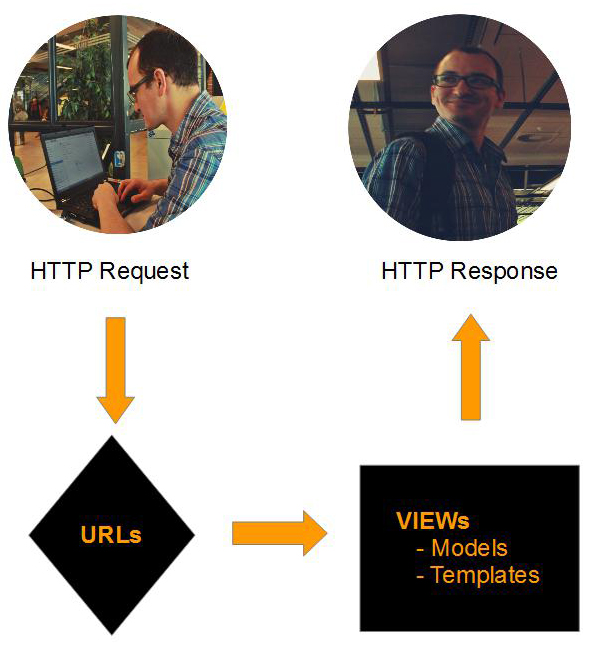
\includegraphics[width=0.55\textwidth]{MVC.jpg}
	\end{center}
	}






\end{document}